\subsection{Barrier options: a modern approach}\lesson{22}{29/04/2020} % Bjork
Let's consider a Wiener process with drift $\mu$ and diffusion $\sigma$ starting at point $\alpha$, i.e.
\begin{equation}
    \begin{cases}
    \dd X(t) = \mu \dd t + \sigma \dd W(t) \\
    X(0) = \alpha
    \end{cases}
\end{equation}
and a hitting time
\begin{equation}
    T_{\beta} = \inf\{t\ge0:X(t)=\beta\}
\end{equation}
\begin{definition}[Absorbed process]
    The $X$-process \emph{absorbed at} $\beta$ is defined by
    \begin{equation}
        X(t\wedge T_{\beta}) = \begin{cases}
        X(t) & t < T_{\beta} \\
        \beta & t \ge T_{\beta}
        \end{cases}
    \end{equation}
\end{definition}
\begin{figure}[h]
    \centering
    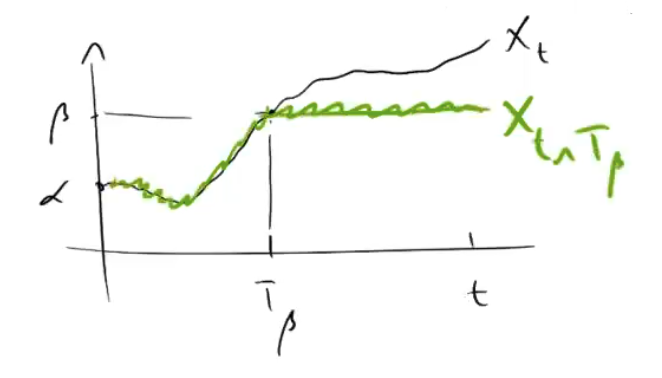
\includegraphics[scale=0.25]{fig/tmp/fig37.png}
    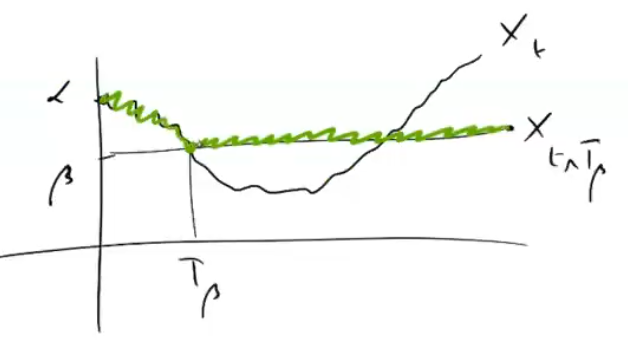
\includegraphics[scale=0.25]{fig/tmp/fig38.png}
    \caption{Absorbed process (a) for $\beta>\alpha$ (b) for $\beta<\alpha$.}
    \label{fig:absproc}
\end{figure}
We are primarily interested in the one-dimensional marginal distribution for $X(t\wedge T_{\beta})$, i.e. the distribution at time $t$ of the $X$-process, absorbed at the point $\beta$. The distribution of $X(t\wedge T_{\beta})$ is of course a mixed distribution in the sense that it has a point mass at $x = \beta$ (the probability that the process is absorbed prior to time $t$) and a density:
\begin{equation}
    f_{X(t\wedge T_{\beta})} = \text{density} + \text{mass in }X= \beta
\end{equation}
This density has its support on the interval $(\beta,\infty)$ if $\alpha > \beta$, whereas the support is the interval $(-\infty,\beta)$ if $\alpha < \beta$.
\begin{definition}[Density of a normal distribution]
    Let $\varphi(x;\mu, \sigma)$ denote the density of a normal distribution with mean $\mu$ and variance $\sigma^2$, i.e.
    \begin{equation}
        \varphi(x;\mu, \sigma) = \frac{1}{\sigma\sqrt{2\pi}}\exp{-\frac{(x-\mu)^2}{2\sigma^2}}
    \end{equation}
\end{definition}
\begin{proposition}\label{f}
    The density $f_{\beta}(x;t,\alpha)$ of the absorbed process $X(t\wedge T_{\beta})$ is given by
    \begin{equation}\label{opopoopopo}
        f_{X(t\wedge T_{\beta})}(x;t,\alpha) = \varphi(x;\mu t+ \alpha, \sigma\sqrt{t})-\exp{-\frac{2\mu(\alpha-\beta)}{\sigma^2}}\varphi(x;\mu t - \alpha + 2\beta, \sigma\sqrt{t})
    \end{equation}
    The support of this density is the interval $(\beta,\infty)$ if $\alpha > \beta$, and the interval $(-\infty,\beta)$ if $\alpha < \beta$.
\end{proposition}

\subsubsection{Down-and-out contracts}
Let's apply this result in a B\&S market with
\begin{equation}
    \begin{cases}
    \frac{\dd S(t)}{S(t)} = r\,\dd t + \sigma\, \dd W^{\Qmeas}(t) \\
    \frac{\dd S(0)}{S(0)} = r\,\dd t
    \end{cases}
\end{equation}
We are interested in pricing a particular contract. Fix a real number $L < S(0)$, which will act as the barrier, and consider the following contract, which we denote by $Z_{LO}$:
\begin{itemize}
    \item If the stock price stays above the barrier L during the entire contract period, then the amount Z is paid to the holder of the contract.
    \item If the stock price, at some time before the delivery time T, hits the barrier L, then the contract ceases to exist, and nothing is paid to the holder of the contract.
\end{itemize}
The contract $Z_{LO}$ is called the “down-and-out” version of the contract $Z$ above, and our main problem is to price $Z_{LO}$. More formally we can describe $Z_{LO}$ as:
\begin{equation}
    Z_{LO} = \Phi(S(T))\mathds{1}_{S(T)<L} = \begin{cases}
    \Phi(S_T) & \text{if } S(t)>L\,\,\forall t\in[0,T] \\
    0 & \text{otherwise}
    \end{cases}
\end{equation}
Concerning the notation, $L$ as a subscript indicates a ``down"-type contract, whereas the letter $O$ indicates that we are considering an ``out" claim.
\begin{theorem}[Pricing down-and-out contracts]\label{daoprice}
    The pricing function, denoted by $F_{LO}$, of a down-and-out contract $Z_{LO}$ is given by
    \begin{equation}\label{uiuiuiu}
        F_{LO}(t,S(t)=s,\Phi) = \left[F(t,s,\Phi_L) - \left(\dfrac{L}{s}\right)^{\frac{2\left(r-\tfrac{\sigma^2}{2}\right)}{\sigma^2}}F\left(t,\frac{L^2}{s},\Phi_L\right)\right]\mathds{1}_{s>L}
    \end{equation}
    where
    \begin{equation}
        \Phi_L(X) = \Phi(X)\mathds{1}_{x>L}. % Phi = payoff
    \end{equation}
\end{theorem}
Notice that the indicator function $\mathds{1}_{x>L}$ represents an European-style barrier, because it involves the terminal value of the underlying. So, this theorem tells us that the price of the barrier option can be written as a combination of prices of the usual European options.
\begin{proof}
    Without loss of generality we may set $t = 0$. Assume then that $S(0) = s > L$, and recall that $S(T\wedge T_L)$ denotes the process $S$ with (possible) absorption at $L$. Using the risk neutral valuation we have:
    \begin{align*}
        F_{LO}(0,S(0)=s,\Phi) &= e^{-rT}\expect_{0,s}[Z_{LO}] = e^{-rT}\expect_{0,s} \left[\Phi(S(T))\mathds{1}_{\inf_{0\le t\le T}S(t)>L}\right] \\
        &=
        e^{-rT}\expect_{0,s}\left[\Phi_L(S(T\wedge T_L))\mathds{1}_{\inf_{0\le t\le T}S(t)>L}\right] \\
        &=
        e^{-rT}\expect_{0,s}[\Phi_L(S(T\wedge T_L))] \\
        \overset{(a)}&{=}
        e^{-rT}\int_L^{\infty}\Phi_L(x)h(x)\,\dd x
    \end{align*}
    where $h(x)$ is the density function for the stochastic variable $S(T\wedge T_L)$. From the theory we know that
    \begin{align*}
        S(T) &= se^{\left(r-\frac{\sigma^2}{2}\right)T+\sigma W^{\Qmeas}(T)} \\
        &=
        e^{\ln s + \Tilde{r}T + \sigma W^{\Qmeas}(T)} = e^{X(T)}
    \end{align*}
    where we used the notation $\Tilde{r} = r - \tfrac{\sigma^2}{2}$ and where the process $X$ is defined by
    \begin{equation*}
        \begin{cases}
        \dd X(t) = \Tilde{r}\,\dd t + \sigma\dd W(t)\\
        X(0) = \ln s
        \end{cases}
    \end{equation*}
    Thus we have
    \begin{equation*}
        S(T\wedge T_L) = e^{X(t\wedge T_{\ln L})}
    \end{equation*}
    so we may write
    \begin{equation*}
        \expect_{0,s}[\Phi_L(S(T\wedge T_L))] = \int_{\ln L}^{\infty} \Phi_L(e^x)f(x)\,\dd x
    \end{equation*}
    where $f$ is the density of the stochastic variable $X(t\wedge T_{\ln L})$. This density is, however, given by Proposition \ref{f} as
    \begin{align*}
        f(x) &= \varphi\left(x;\Tilde{r}T+\ln s,\sigma\sqrt{T}\right) - \\
        &\qquad\qquad - \exp{-\frac{2\Tilde{r}(\ln s - \ln L)}{\sigma^2}}\varphi\left(x;\Tilde{r}T-\ln s+2\ln L, \sigma\sqrt{T}\right) \\
        &=
        \varphi\left(x;\Tilde{r}T+\ln s,\sigma\sqrt{T}\right) - \left(\frac{L}{s}\right)^{\frac{2\Tilde{r}}{\sigma^2}}\varphi\left(x;\Tilde{r}T+\ln \left(\frac{L^2}{s}\right), \sigma\sqrt{T}\right)
    \end{align*}
    Thus we have
    \begin{align*}
        \expect_{0,s}[\Phi_L(S(T\wedge T_L))] &= \int_{\ln L}^{\infty} \Phi_L(e^x)f(x)\,\dd x \\
        &=
        \int_{\ln L}^{\infty}\Phi_L(e^x)\varphi\left(x;\Tilde{r}T+\ln s,\sigma\sqrt{T}\right) - \\ % fine parte 1
        &\qquad\qquad
        - \left(\frac{L}{s}\right)^{\frac{2\Tilde{r}}{\sigma^2}} \int_{\ln L}^{\infty}\Phi_L(e^x) \varphi\left(x;\Tilde{r}T+\ln \left(\frac{L^2}{s}\right), \sigma\sqrt{T}\right)\,\dd x \\
        &=
        % i can extend the integral in R thanks to the presence of the indicator function
        \int_{\mathbb{R}} \Phi_L(e^x) \varphi\left(x;\Tilde{r}T+\ln s,\sigma\sqrt{T}\right) \,\dd x - \\
        &\qquad\qquad
        - \left(\frac{L}{s}\right)^{\frac{2\Tilde{r}}{\sigma^2}} \int_{\mathbb{R}} \Phi_L(e^x) \varphi\left(x;\Tilde{r}T+\ln \left(\frac{L^2}{s}\right), \sigma\sqrt{T}\right)\,\dd x
    \end{align*}
    Inspecting the last two lines we see that the density in the first integral is the density of $X(T)$ under the usual martingale measure $\Qmeas$, given the starting value $S(0) = s$. The density in the second integral is, in the same way, the density (under $\Qmeas$) of $X(T)$, given the starting point $S(0) = L^2/s$. Thus we have
    \begin{equation*}
        \expect_{0,s}[\Phi_L(S(T\wedge T_L))] = \expect_{0,s}[\Phi_L(S(T))] - \left(\frac{L}{s}\right)^{\frac{2\Tilde{r}}{\sigma^2}} \expect_{0,\frac{L^2}{s}}[\Phi_L(S(T))]
    \end{equation*}
    which gives us the pricing function
    \begin{align*}
        F_{LO}(0,s,\Phi) &= e^{-rT}\expect_{0,s}[\Phi_L(S(T))] - e^{-rT}\left(\frac{L}{s}\right)^{\frac{2\Tilde{r}}{\sigma^2}} \expect_{0,\frac{L^2}{s}}[\Phi_L(S(T))] \\
        &=
        \left[F(t,s,\Phi_L) - \left(\dfrac{L}{s}\right)^{\frac{2\Tilde{r}}{\sigma^2}}F\left(t,\frac{L^2}{s},\Phi_L\right)\right]\mathds{1}_{s>L}
    \end{align*}
\end{proof}
We again emphasize the point of this result: the problem of computing the price for a down-and-out claim reduces to the standard problem of computing the price of an ordinary (related) claim without a barrier.\\
We also note the fact that down-and-out pricing is a linear operation.
\begin{corollary}\label{linearitycor}
    For any contract payoffs $\Phi$ and $\Psi$, and for any real numbers $\alpha$ and $\beta$, the following relation holds:
    \begin{equation}
        F_{LO}(t,s,\alpha\Phi+\beta\Psi) = \alpha F_{LO}(t,s,\Phi) + \beta F_{LO}(t,s,\Psi).
    \end{equation}
\end{corollary}
\begin{proof}
    The result follows immediately from Theorem \ref{daoprice} together with the linearity of the ordinary pricing functional $F$ and the linearity of the chopping operation:
    \begin{align*}
        (\alpha\Phi(x)+\beta\Psi(x))_L &= (\alpha\Phi(x)+\beta\Psi(x))\mathds{1}_{x>L} \\
        &=
        \alpha\Phi(x)\mathds{1}_{x>L} + \beta\Psi(x)\mathds{1}_{x>L} \\
        &=
        \alpha\Phi(x)_L + \beta\Psi(x)_L
    \end{align*}
\end{proof}

\subsubsection{Up-and-out contracts}
We now describe the up-and-out version of $Z$. This is the contract which at the time of delivery, $T$, will pay $Z$ if the underlying price process during the entire contract period has stayed below the barrier $L$. If, at some time during the contract period, the price process exceeds $L$, then the contract is worthless. In formal terms this reads as follows.
\begin{equation}
    Z^{LO} = \Phi(S(T))\mathds{1}_{S(t)<L\,\forall t\in[0,T]} =
    \begin{cases}
    \Phi(S(T)) & \text{if } S(t)<L\,\,\forall t\in[0,T] \\
    0 & \text{otherwise}
    \end{cases}
\end{equation}
The pricing functional for $Z^{LO}$ is denoted by $F^{LO}(t,s,\Phi)$.\\
$L$ as a superscript indicates an ``up"-type contract, whereas the superscript $O$ indicates that the contract is an ``out" contract. As in the previous section we will relate the up-and-out contract to an associated standard contract.
\begin{theorem}[Pricing up-and-out contracts]
    Consider a fixed $T$-claim $Z = \Phi(S(T))$. Then the pricing function, $F^{LO}$, of the corresponding up-and-out contract $Z^{LO}$ is given by
    \begin{equation}\label{uaoprice}
        F^{LO}(t,s,\Phi) =
        \left[F(t,s,\Phi^L) - \left(\dfrac{L}{s}\right)^{\frac{2\Tilde{r}}{\sigma^2}}F\left(t,\frac{L^2}{s},\Phi^L\right)\right]\mathds{1}_{s<L}
    \end{equation}
    with
    \begin{equation}
        \Phi^L =
        \begin{cases}
        \Phi(x) & \text{for }x<L \\
        0 & \text{for }x\ge L
        \end{cases},
        \qquad \Tilde{r} = r - \frac{\sigma^2}{2}.
    \end{equation}
\end{theorem}
\begin{remark}
    From eqs. \eqref{uiuiuiu} and \eqref{uaoprice} we see that the price of a barrier option is given by a difference between the price of a contract and the price of a modified version of the same contract, which is positive. This means that a barrier option is cheaper than the corresponding vanilla option (for example a barrier call option will be cheaper than a vanilla call). On the other hand, entering a barrier option in order to hedge is dangerous, because if the underlying touches the barrier then there every possibility to hedge is lost.
\end{remark}

\subsubsection{Examples}
Let us define the following standard contracts, which will be the basic building blocks in the sequel. Fix a delivery time $T$. For fixed parameters $K$ and $L$ define the following claims:
\begin{itemize}
    \item $ST(x) = x$ is the payoff which gives (the price of) one unit of the underlying stock at delivery time $T$. Basically, it is a long position on the underlying $S(t)$;
    \item $BO(x) = 1$ is an ordinary zero coupon bond paying one at maturity $T$;
    \item $H(x,L) = \mathds{1}_{x>L}$ gives the owner one if the value of the underlying stock exceeds $L$ at delivery time $T$, otherwise nothing is paid out (digital call);
    \item $C(x,K) = (x-K)^+$ is the ordinary European call with strike price $K$.
\end{itemize}
We now list the pricing functions for the standard contracts above.
\begin{itemize}
    \item the value of $ST$ at time $t$ is equal to the value of the
    underlying stock at the same time:
    \begin{equation}
        ST(t,S(t)=s) = price_t(ST) = e^{-r(T-t)}\expect_{t,s}[S(T)] = S(t) = s
    \end{equation}
    \item the value of $BO$ at time $t$ is
    \begin{equation}
        BO(t,s) = price_t(BO) = e^{-r(T-t)}
    \end{equation}
    \item the value of $H$ is calculated by using the risk neutral methodology:
    \begin{align}
        \notag H(t,s,L) &= price_t(H(S(T),L) = e^{-r(T-t)}\Phi(d_2) \\
        &=
        e^{-r(T-t)}\Phi\left(\frac{\Tilde{r}(T-t) + \ln(\tfrac{s}{L})}{\sigma\sqrt{T-t}}\right)
    \end{align}
    \item The value of $C$ is given by the B\&S formula.
\end{itemize}
Notice that
$$BO_L(x) = 1\cdot\mathds{1}_{x>L} = H(x,L).$$
